\documentclass[letterpaper,journal]{IEEEtran}
\usepackage{amsmath,amssymb,amsfonts,array,booktabs,tabularx}
\usepackage{graphicx,xcolor,algorithm,algorithmic,tikz,cite,url}
\usepackage{microtype}
\usetikzlibrary{arrows.meta,positioning,fit}
\usepackage[hidelinks]{hyperref}
\hypersetup{pdftitle={FreqDuet: Cumulative Holding Budgets for Fixed-Fleet Timetable Coordination},pdfauthor={Anonymous Authors}}
\newcommand{\E}{\mathbb{E}}
\newcommand{\clip}{\operatorname{clip}}
\newcommand{\pos}[1]{[#1]_+}
\newcolumntype{Y}{>{\raggedright\arraybackslash}X}
\newcommand{\ManualBudgetGain}{2.396}
\newcommand{\ManualReadinessGain}{4.540}
\newcommand{\ManualBudgetCV}{+0.003025}
\newcommand{\LearnedBudgetGain}{1.645}
\newcommand{\HarmonicJourney}{-0.562}
\newcommand{\HarmonicCV}{-0.000937}
\newcommand{\PressureStaticGain}{3744.15}
\newcommand{\PressureCapGain}{3123.80}
\newcommand{\JointStaticLoss}{6.803}
\newcommand{\JointCapLoss}{10.744}

\hyphenation{time-table time-tables co-or-di-na-tion}
\begin{document}
\title{FreqDuet: Cumulative Holding Budgets for Fixed-Fleet Timetable Coordination}
\author{Anonymous Authors}
\markboth{RESEARCH DRAFT, NOVEMBER 2026}{Cumulative Holding Budgets and Vehicle Circulation}
\maketitle
\begin{abstract}
Terminal timetable revisions and en-route holding compete for the same vehicle time. We study their coordination through persistent trip-level holding budgets shared by forecasting, legal-action enumeration, and physical execution. The system combines causal demand summaries, a bounded timetable law, and a model-based fast controller; a learned publication-permission policy is evaluated separately. On 16 independent simulation demand days, reducing the manual joint controller's budget retention from 0.50 to 0.25 reduced restricted journey exposure by \ManualBudgetGain\ s/passenger and readiness delay by \ManualReadinessGain\ s/trip, while increasing actual headway CV$^2$ by \ManualBudgetCV. On another 16 new days, pressure-driven credit reduced daily public dispatch delay by \PressureStaticGain\ s relative to a static-credit mixture and by \PressureCapGain\ s relative to a stop-cap mixture calibrated on development holding exposure. Both comparisons worsened actual CV$^2$ and failed the prespecified joint criterion. A common-reference credit-admission redesign restored regularity on four further development days but increased journey exposure by \JointStaticLoss\ and \JointCapLoss\ s/passenger relative to the simple controls. Matched-budget comparisons did not establish a learned-supervisor journey advantage, and the independent harmonic-journey criterion also failed. The evidence supports an executable, configurable vehicle-time interface and reproducible operational tradeoffs, rather than a demonstrated improvement over simple limits at preserved regularity.
\end{abstract}
\begin{IEEEkeywords}
Bus holding, timetable coordination, vehicle circulation, cumulative time budgets, model-based control, paired simulation.
\end{IEEEkeywords}
\section{Introduction}
\IEEEPARstart{H}{olding} a bus can improve service spacing while delaying the passengers already on board. Under a fixed fleet, the same seconds can also postpone the vehicle's next departure. A terminal timetable revision therefore depends not only on demand and the current terminal queue, but also on how much vehicle time downstream holding will consume. This study examines that connection through a shared cumulative holding budget.

The service--holding tradeoff is established in the bus-control literature. Daganzo's headway-based control seeks reliable high-frequency service with reduced schedule slack~\cite{daganzo2009headway}. Daganzo and Pilachowski extend cooperation to front and rear spacing, using speed adjustment to counter large gaps~\cite{daganzo2011cooperation}. Berrebi \emph{et al.} compare predictive and non-predictive holding methods in terms of headway stability and holding time~\cite{berrebi2018comparing}. These findings motivate a direct question: does a turnover-aware allocation rule improve the operating tradeoff relative to simple holding restrictions, or does it mainly choose a different point on that tradeoff?

An executable comparison requires consistent resource semantics. A timetable predictor can assume a returning vehicle will be available while later holding delays that return. A cumulative allowance can also have different effects from a per-stop cap even when both lead to similar average holding. We address these issues by using the same published releases, irreversible commands, and remaining-credit ledger inside each forecast and in physical execution. This makes a budget an inspectable resource constraint rather than an additional reward term.

The architecture also permits a controlled examination of temporal information and learning. Causal harmonic summaries inform a bounded timetable law; the fast layer evaluates legal holding actions on current automatic passenger count (APC) and automatic vehicle location (AVL) observations. A learned supervisor can enable or withhold timetable revisions, but the same interface can be driven by an always-joint manual supervisor. Matching their budget settings separates a learning increment from a change in holding exposure. Matching a harmonic and non-harmonic representation addresses a different question again.

We present three contributions. First, we specify the time-budget interface and its accounting invariants under a fixed fleet and a fixed trip roster. Second, independent paired-demand experiments establish how retention changes passenger exposure, circulation, and actual regularity, while separating those effects from supervisor choice. Third, strong simple-limit comparisons and a common-reference admission redesign expose the present boundary of pressure-driven allocation. The resulting evidence identifies both an operationally useful configuration effect and the unresolved challenge of improving it without transferring cost to service regularity.

\section{Related Work}
\subsection{Holding, Prediction, and Vehicle Circulation}
Headway-based regulation uses spacing information to control unstable service~\cite{daganzo2009headway}. Cooperative control can additionally exploit the state of the following bus~\cite{daganzo2011cooperation}. The native continuation used here is a discrete bilateral holding rule; it is not the continuous speed controller of Daganzo and Pilachowski. Its availability provides a defined fallback when the event model lacks support.

Prediction-based holding introduces a further distinction between the action preferred under a forecast and its realized service effect. The predictive/non-predictive comparison of Berrebi \emph{et al.}~\cite{berrebi2018comparing} is particularly relevant to assessing headway stability alongside the intervention time required. Our comparison adds a fixed physical vehicle pool, public departure obligations, and a cumulative allowance that can affect both return forecasts and executable commands. The tests retain simple credit and stop-cap controls rather than interpreting improvement over an old learner as sufficient evidence.

Asynchronous multi-agent reinforcement learning addresses the non-simultaneous decisions made when different buses reach stops~\cite{wang2021asynchronous}. Our fast decisions are also event-triggered, but are selected by finite model-based enumeration. The optional learned component instead acts on the slow publication clock. This distinction matters for interpreting which component is responsible for an observed operating change.

\subsection{Temporal Representation and Action Persistence}
Multiple control frequencies can be formalized through action persistence, including policies whose action components operate on different clocks~\cite{lee2020multiple}. Persistence can itself be adapted or optimized in batch reinforcement learning~\cite{metelli2020persistence}. A persistent holding allowance is a resource commitment across stop events; it is not repeated execution of one fixed holding command.

Similarly, a harmonic representation of observations is not equivalent to frequency-specific action authority. Here, harmonic summaries enter the slow state and timetable law. The fast layer uses APC clearance evidence, AVL, plans, and remaining credit. The representation comparison therefore tests a defined change to this implementation, not a complete separation of low- and high-frequency controllers. The learned comparator uses a finite-action maximum-entropy actor--critic~\cite{haarnoja2018sac,christodoulou2019discrete}; its optimizer is retained as an experimental component rather than a claimed methodological advance.

\section{Problem and Information Structure}
\label{sec:problem}
Consider a bidirectional bus service with a fixed fleet and a fixed set of trips $\mathcal T$. Trip $j$ has a public reference departure $p_j$, an operationally published release $\tau_j$, and an actual departure $d_j$. Public references remain unchanged when the controller revises a release. Each controllable stop visit $e$ receives a holding command $h_e$ from a finite legal set $\mathcal H_e$. Vehicle returns determine the supply available to later trips, so the feasible schedules and holding sequences are coupled.

Let $W$ and $R$ denote total passenger waiting and on-board time, respectively, in person-seconds. The accounting includes the prescribed tail of service and uses the same generated passenger population for paired policies. Let $D_{\mathrm{pub}}$ be total positive departure delay measured against the immutable public references. The implemented upper objective is
\begin{equation}
 J_0=\frac{W+R}{3{,}600{,}000}+\frac{D_{\mathrm{pub}}}{94{,}320}.
 \label{eq:objective}
\end{equation}
The fixed divisors define the relative scale used to train the optional learned supervisor. The manual supervisor applies the timetable and budget laws directly; it does not minimize this composite by learning. The fast model minimizes predicted $W+R$. Actual passenger exposure, public dispatch delay, readiness, and CV$^2$ are evaluated separately under each study's frozen hypotheses.

At decision time $t$, the controller uses a history $\mathcal I_t$ consisting of available APC events, AVL telemetry, completed-trip summaries, and published plans. APC fields include time, station, direction, boarding and alighting counts, and entering load. Completion of a service event can occur after its arrival observation. Historical statistics requiring completed service are formed only after completion; currently available events can already inform queue reconciliation. Simulator passenger records are used to score physical outcomes, not to fill an unobserved current queue in the predictive graph.

The distinction between boarding and arrival rates is operationally consequential. A vehicle with spare capacity that serves the waiting passengers provides a clearance observation. A full vehicle gives a censored observation of demand: the number boarded does not determine the number remaining. Between clearance events, a model may propagate a queue using an estimated arrival rate, but that propagation remains a forecast. The controller cannot infer that no passenger arrived merely because no bus boarded passengers during the interval.

\section{Timetable and Holding-Budget Interface}
\label{sec:method}
\begin{figure*}[t]
\centering
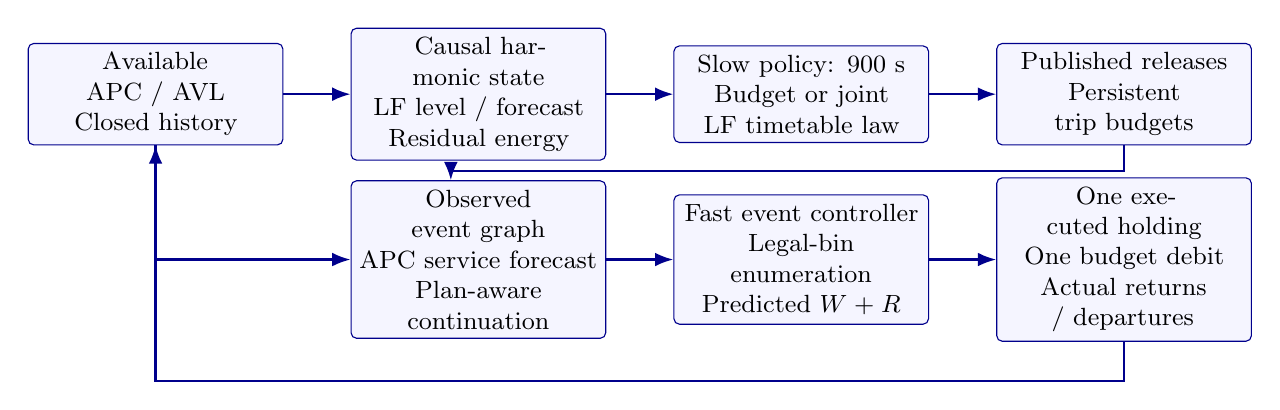
\begin{tikzpicture}[font=\small,>=Latex,
 box/.style={draw=blue!55!black,rounded corners=2pt,fill=blue!4,align=center,minimum height=1.0cm,text width=3.0cm},
 arr/.style={->,thick,blue!55!black}]
\node[box] (data) at (0,0) {Available APC / AVL\\Closed history};
\node[box] (freq) at (4.1,0) {Causal harmonic state\\LF level / forecast\\Residual energy};
\node[box] (slow) at (8.2,0) {Slow policy: 900 s\\Budget or joint\\LF timetable law};
\node[box] (ledger) at (12.3,0) {Published releases\\Persistent trip budgets};
\node[box] (graph) at (4.1,-2.1) {Observed event graph\\APC service forecast\\Plan-aware continuation};
\node[box] (fast) at (8.2,-2.1) {Fast event controller\\Legal-bin enumeration\\Predicted $W+R$};
\node[box] (physical) at (12.3,-2.1) {One executed holding\\One budget debit\\Actual returns / departures};
\draw[arr] (data)--(freq);
\draw[arr] (freq)--(slow);
\draw[arr] (slow)--(ledger);
\draw[arr] (data.south) |- (graph.west);
\draw[arr] (ledger.south) -- ++(0,-.32) -| ([xshift=-.35cm]graph.north);
\draw[arr] (graph)--(fast);
\draw[arr] (fast)--(physical);
\draw[arr] (physical.south) -- ++(0,-.5) -| (data.south);
\end{tikzpicture}
\caption{Shared information and resource interface, reused from the development architecture. Manual joint fixes the slow mode to joint; the learned comparator selects budget or joint. The fast controller uses APC/AVL, published plans, and remaining budgets. Frequency summaries enter the slow state and timetable law. Physical events update observations and resource accounting.}
\label{fig:architecture}
\end{figure*}

\subsection{Causal Frequency Summaries}
The frequency tracker forms closed-bin APC signals and maintains a causal harmonic state. For a nonnegative observed rate $x_n$, let $z_n=\log(1+x_n)$ and let $\phi_n$ contain an intercept, a temporal trend, and harmonic basis terms. A recursive least-squares update has the form
\begin{align}
 k_n&=\frac{P_{n-1}\phi_n}{\rho+\phi_n^\top P_{n-1}\phi_n},\\
 \theta_n&=\theta_{n-1}+k_n(z_n-\phi_n^\top\theta_{n-1}),\\
 P_n&=\rho^{-1}(P_{n-1}-k_n\phi_n^\top P_{n-1}).
\end{align}
Here $\rho$ is the recursive estimator's forgetting factor, distinct from budget retention $\rho_B$. The transformed fitted value supplies a nonnegative low-frequency (LF) summary $L_n$. A residual is formed against the \emph{pre-update} prediction, and its smoothed value and high-frequency (HF) energy are retained. Thus the fitted low component and smoothed residual are not an exact additive reconstruction of the raw count. A future LF summary is obtained by evaluating the fitted state at the future harmonic phase, without incorporating future observations.

The implemented slow state includes global low demand, its slope, a low-frequency forecast, and high-frequency energy. The timetable rule uses the global low level and forecast. Station-specific short-window arrival-rate estimates in the fast graph are obtained separately from APC clearance intervals. They have units of passengers per second and are not interchangeable with boarding-bin residuals. This separation avoids adding quantities with different sampling and exposure meanings.

\subsection{Bounded Dynamic Timetable Revision}
The slow manager begins at 7200 s and considers publication every 900 s. For each direction, a revision concerns the next mutable departure and preserves the following departure as an anchor. Write $p_1$ for the next public release, $p_2$ for the following public release, and $d_-$ for the preceding actual departure. Let $L_t$ and $F_t$ be the currently supported low-frequency level and forecast. Define
\begin{align}
 \omega_t&=\clip((p_2-t)/1800,0,1),\\
 \ell_t&=\pos{L_t},\qquad r_t=\pos{(1-\omega_t)L_t+\omega_t F_t},\\
 \tau^*&=\frac{\ell_t d_-+r_t p_2}{\ell_t+r_t}.
 \label{eq:timetable}
\end{align}
If the frequency estimate is unsupported, equal weights replace $\ell_t$ and $r_t$. The proposed release is restricted to a $\pm30$ s shift around $p_1$, then constrained by the current time, a 180 s minimum separation from the preceding published release, and a 180 s separation from the anchor. The executable value is rounded upward to the simulator's integer-second clock. Both the revised trip's target headway and the anchor's following target headway are updated.

A revision requires two mutable future departures within the publication window, sufficient completed-trip history, and a compatible vehicle-supply estimate. A trip that has already become operationally committed is not rewritten. The rule evaluates supply from available vehicles and forecast returning vehicles; it does not create an additional vehicle or reserve an unobserved return. Manual joint always enables this law and the budget mechanism. The optional learned supervisor controls permission to invoke the law rather than directly optimizing timetable entries.

\subsection{Persistent Holding Budgets}
For each active vehicle--trip pair $i$, the manager estimates the normal remaining command exposure $C_i$ from the number of remaining controls and the median command seconds per control in at least three completed eligible trips of the same direction. A return estimate separates the remaining non-holding running and service component, irrevocable commands, and the physical overhead of control events. It is matched to an upcoming trip within a 2700 s supply look-ahead.

Let $\widehat r_i^{\mathrm{ord}}$ be the estimated ordinary return time, and $p_{j(i)}$ the public departure of the matched trip. The estimated supply pressure and proposed remaining allowance are
\begin{align}
 P_i&=\pos{\widehat r_i^{\mathrm{ord}}+1-p_{j(i)}},\\
 \widetilde B_i&=\left\lceil\max(\rho_B C_i,C_i-P_i)\right\rceil.
 \label{eq:budget}
\end{align}
The default uses $\rho_B=0.5$; the independent configuration study also evaluates 0.25 without retraining. This retention floor preserves a fraction of the estimated ordinary command exposure; a larger value permits more holding time at the same supply pressure. The ordinary exposure is estimated from the policy's own completed-trip history, not an externally fixed regularity requirement. The allowance is vehicle time, not a vehicle or driver fraction. Only active trips with positive pressure, positive normal exposure, and remaining control opportunities receive a new allowance. If one already exists, publication takes $\min(B_i,\widetilde B_i)$ rather than replenishing it. At final submission of a command,
\begin{equation}
 B_i\leftarrow B_i-h_e,\qquad h_e\leq B_i^{\mathrm{before}}.
 \label{eq:debit}
\end{equation}
The allowance is closed when that trip returns. It persists across changes in the upper mode and across all remaining control points.

Budget accounting uses command seconds. In the simulator, a zero command still occupies one physical tick at a control point. Thus physical residence is $\max(1,h_e)$ for a submitted command, with corresponding automatic zero ticks at unrequested controls. Treating residence as identical to the budget debit would change the executed model. The return predictor estimates this overhead separately; it does not claim that subtracting one budget second always advances a return by one second.

\subsection{Fast Holding with a Common Continuation}
The native bilateral request uses forward departure spacing $g_f$ and a causal estimate of following-bus action-ready spacing $g_b$. When both are supported, its continuous request is $0.25(g_b-g_f)/2$. Without following-bus evidence it uses $0.25(T-g_f)$ for the trip target $T$; without forward evidence it requests zero. The result is clipped to $[0,45]$ s and mapped to the nearest original legal bin, with ties selecting the shorter command. Follower identity and timing use current telemetry and completed observations, not future return labels.

At a controllable event, the fast layer constructs a graph from the same current observations, published plans, and budget ledger. Its reference is the native bilateral rule projected onto the remaining allowance. If the native command is $h_e^{\mathrm{nat}}$, the projection is
\begin{equation}
 \bar h_e=\max\{h\in\mathcal H_e:h\leq h_e^{\mathrm{nat}},\ h\leq B_i\},
 \label{eq:projection}
\end{equation}
where the budget restriction is omitted for an unbudgeted trip. The rule's original legal mask is preserved. The current controller enumerates the legal members of $\{0,5,10,15,20,30,45\}$ s, using the same future native continuation and a separate copy of the ledger for each evaluation. The selected action minimizes predicted $W+R$ over candidates that satisfy the frozen relative feasibility conditions: predicted CV$^2$, relevant vehicle return times, subsequent departure times, and trip departure delays must not exceed their reference values. Coverage must be complete for the required events. The first executable command is applied; future actions remain predictions.

Published releases affect terminal events and downstream supply matching in the graph. Budget depletion changes later available commands. These dependencies mean that the two layers interact through a shared feasible set, even if the immediate passenger-cost ordering of the current holding candidates does not change. Every trial starts from the same remaining allowance, so searching more candidates does not spend physical budget. Only the executed command debits the live ledger.

If the predictive reference lacks the required support, the controller uses the budget-feasible native command. This fallback is an operational part of the method. An enumeration can be exact over the current finite library and still fail to identify the best real-world action, because the future continuation and demand estimates are approximate. We therefore distinguish search completeness from prediction accuracy and from actual transport benefit.

\subsection{Optional Learned Publication-Permission Comparator}
The upper action set is $\mathcal A=\{\mathrm{budget},\mathrm{joint}\}$. Both modes permit persistent budgets; only the joint mode permits a new timetable revision. The 180-dimensional state contains the time, fleet load, frequency summaries, accumulated arrival-headway moments, public-delay debt, the previous mode, directional supply and plan summaries, completed-trip history, and telemetry and remaining allowances for the 12 vehicles. Fixed divisors normalize these fields. The same canonical action labels are used in the actor, critic, replay, previous-action encoding, and execution.

The reward is the negative increment of~\eqref{eq:objective} over a slow interval. With $\gamma=1$ and a finite daily episode, interval increments retain their daily accounting interpretation. The final interval is closed after the service tail. A discrete maximum-entropy actor--critic uses twin critics and the target
\begin{align}
 V(s')&=\sum_{a'}\pi(a'|s')\left[\min_m\bar Q_m(s',a')-\alpha\log\pi(a'|s')\right],\\
 y&=r+(1-d)V(s').
\end{align}
where $d$ denotes termination. The actor minimizes
\begin{equation}
 L_\pi=\E_s\sum_a\pi(a|s)\left[\alpha\log\pi(a|s)-\min_m Q_m(s,a)\right].
\end{equation}
The entropy temperature is fixed at $10^{-5}$, the hidden width is 64, the learning rate is $3\times10^{-4}$, and the target update coefficient is 0.005. Replay capacity is 8192. Training behavior mixes the policy with a 0.1 uniform exploration component; evaluation uses the deterministic policy. These settings are held fixed for the action-semantics comparison.

\begin{algorithm}[t]
\caption{The shared timetable--holding interface}
\label{alg:control}
\begin{algorithmic}[1]
\STATE Update histories from newly available APC/AVL events.
\IF{a new slow publication time has been reached}
\STATE Use joint for manual control, or select budget/joint with the frozen supervisor.
\STATE Issue or tighten trip budgets using~\eqref{eq:budget}.
\IF{joint is selected and a plan revision is supported}
\STATE Publish the bounded release and its two target headways.
\ENDIF
\ENDIF
\IF{a vehicle requests a holding action}
\STATE Build the observed graph with current plans and budgets.
\STATE Project the native reference using~\eqref{eq:projection}.
\STATE Enumerate current legal candidates with separate ledgers.
\STATE Select the lowest-cost feasible action or reference fallback.
\STATE Submit one command and debit its live trip allowance once.
\ENDIF
\STATE Close the allowance when its physical trip returns.
\end{algorithmic}
\end{algorithm}

\subsection{Joint Credit Admission as a Development Candidate}
Pressure credit in~\eqref{eq:budget} restricts the continuation before the fast model checks relative feasibility. We therefore evaluate a separate candidate that treats new credit itself as a decision. At the slow clock, the original formula proposes an allowance without imposing it. At the proposing cycle's next supported holding query, the unchanged fast selector with existing credit produces a common no-new-tightening reference. We enumerate current legal commands under the proposed credit and require their continuations to meet the same reference's passenger-cost, CV$^2$, return, next-launch, and dispatch-delay conditions. The lowest predicted passenger cost is preferred; exact cost ties prefer lower total public delay. Only a strict cost or delay improvement admits the new allowance.

Commands submitted between proposal and admission debit the proposed remainder. A request expires at the next publication or physical return. Unsupported evidence imposes no new tightening; existing credit and irreversible commands remain unchanged. The chosen allowance is committed before its current command is submitted. This candidate changes credit admission, not the demand predictor, legal bins, cost weights, or fleet.

\subsection{Operational Coupling}
The architecture makes two interactions explicit: slow releases alter fast resource feasibility, and fast holding consumes vehicle time that constrains later releases. It also exposes a useful distinction between \emph{permission} and \emph{dose}. Selecting joint does not guarantee that a plan will be revised; the law may reject a publication, produce the same integer-second release, or be unable to influence an already committed trip. An upper action count is therefore insufficient evidence of timetable control. We record published revisions, binding to actual departures, and changes relative to matched control paths.

The implemented frequency pathway runs from the causal summary to the slow state or timetable law, and then from published plans and budgets to fast control. The architecture in Fig.~\ref{fig:architecture} depicts these paths. The representation and supervisor comparisons evaluate their incremental effects separately from the budget-setting contrast.

\section{Properties of the Coordination Interface}
\label{sec:properties}
The interface admits several limited statements that help interpret the experiments. They concern the meaning of the executed commands and comparisons, rather than optimality of the learned policy.

\subsection{Cumulative Feasibility of a Trip Budget}
Suppose a trip first receives allowance $B_0\geq0$. Let $h_1,\ldots,h_m$ be its subsequently committed holding commands and let $u_1,\ldots,u_q\geq0$ be the reductions imposed by later budget publications. If each command is constrained by the currently remaining allowance and debited exactly once, then
\begin{equation}
 B_{\mathrm{rem}}=B_0-\sum_{e=1}^{m}h_e-\sum_{v=1}^{q}u_v\geq0.
 \label{eq:budget_identity}
\end{equation}
This follows by induction over the ordered sequence of command submissions and publications. A legal submission subtracts at most the current remainder. A publication replaces the remainder by the minimum of itself and a nonnegative proposal, subtracting a nonnegative reduction. Neither event increases the allowance. Consequently, total committed holding after issuance cannot exceed $B_0$, regardless of how often the upper mode changes.

The same identity holds inside an individual predictive continuation because its ledger uses the same events. It does not imply a realized return-time bound: uncertain running and service times, control-point residence, and later dispatch availability remain outside this scalar accounting identity. It also does not compare total holding with an unconstrained policy that would visit different future states. Its practical value is that prediction and execution refer to the same limited resource.

\subsection{Timetable Revision Redistributes Adjacent Targets}
Let $\tau_-$ be the preceding published release. Before a permitted revision, the two adjacent target headways are $p_1-\tau_-$ and $p_2-p_1$. After changing the next release to $\tau_1$, they become $\tau_1-\tau_-$ and $p_2-\tau_1$. Therefore,
\begin{equation}
 (\tau_1-\tau_-)+(p_2-\tau_1)=p_2-\tau_-.
 \label{eq:anchor}
\end{equation}
The law redistributes service within a fixed anchored span. It neither inserts a trip nor increases the nominal fleet. The term ``frequency-informed'' refers to temporal components of the observed signal, rather than an increase in the total scheduled service frequency. As actual releases depend on vehicle availability,~\eqref{eq:anchor} describes published targets and does not force realized headways to attain those values.

This limited intervention also explains why many budget and joint choices can be behaviorally identical. The same state may yield no mutable departure, an unsupported supply estimate, an unchanged rounded release, or a release whose effect is absorbed before dispatch. A critic trained on the mode label then learns across both effective and ineffective interventions. The relevant learning question is whether state information identifies the occasions on which a permitted revision changes passenger outcomes, not whether the actor selects joint often.

\subsection{Identical Cost Rankings Can Produce Different Actions}
Let $\widehat C(h)$ be the predicted passenger cost of a current action, and let $\mathcal F(\tau,B)$ be its feasible set under the published plan and remaining budget. The fast decision is
\begin{equation}
 h^*(\tau,B)\in\arg\min_{h\in\mathcal F(\tau,B)}\widehat C(h).
\end{equation}
Even if a plan change leaves $\widehat C(h_1)<\widehat C(h_2)$ intact, it can switch the selected action by removing $h_1$ from the feasible set. This is operational coupling, not by itself a passenger-cost improvement. The experiments therefore evaluate complete realized trajectories rather than interpreting changed plan or command counts as a benefit.

\subsection{Consistent Windows for Regularity Comparisons}
For $n$ included arrival headways with sum $S$ and squared sum $Q$, the population-moment convention gives
\begin{equation}
 \mathrm{CV}^2=\frac{nQ}{S^2}-1,\qquad n>0,\ S>0.
 \label{eq:cv_moments}
\end{equation}
The fast model extends the actual nonterminal arrival prefix with a predicted suffix. Already observed arrivals are counted once, and terminal returns are excluded from the regularity statistic while remaining in the resource calculation. Complete-day evaluation uses the physical arrival recorder with the same population-moment convention.

\subsection{A Relative Guard Does Not Protect Its Reference}
In the original interface, the fast reference already includes published credit. An action satisfying a non-increasing predicted CV$^2$ condition relative to that reference does not establish that issuing the credit was itself harmless. The joint-admission candidate instead compares the credit restriction and current action against a common no-new-tightening continuation. These are different comparisons even with identical demand forecasts and clocks. Neither comparison is a mathematical guarantee of complete-day non-harm under later closed-loop decisions.

Together, these properties locate the method's guarantees at the interface: cumulative command feasibility, anchored plan semantics, and well-defined comparisons. Realized waiting-time improvement, vehicle readiness, and generalization remain empirical questions.

\section{Experimental Design}
\label{sec:experiments}
\subsection{Physical Contract and Endpoints}
All four studies retained 12 physical vehicles and 262 scheduled trips, with 131 departures per direction at a public 360-s interval. The two directional schedules began 180 s apart. The simulator advanced in 1-s steps; the original seven holding bins were retained throughout. Demand was generated from the frozen hourly origin--destination template with stochastic demand perturbations. A demand-day identifier denotes a simulated realization, not an observed calendar service day.

Demand generation ended at 46,980 s. The evaluation contract allowed a 14,400-s service tail and a maximum horizon of 61,380 s, with earlier physical termination when service cleared. For $N$ passengers generated on the common demand realization, waiting and onboard exposure were $W/N$ and $R/N$. We call their sum \emph{restricted journey exposure}. It includes accounted waiting by generated passengers who remain unserved, rather than conditioning on completed journeys.

For public release $p_j$, actual departure $d_j$, and the observed time $e_j$ when the trip first became dispatch-eligible under its operational plan, the reported operational measures were
\begin{align}
 D_{\rm pub}&=\sum_{j\in\mathcal T}\max(0,d_j-p_j),\\
 \overline D_{\rm ready}&=\frac{1}{262}\sum_{j\in\mathcal T}(d_j-e_j).
\end{align}
Public delay is a daily total; readiness delay is seconds per scheduled trip. The public references were immutable, so changing an operational release could not redefine away measured lateness. Positive public delay does not penalize an early departure symmetrically. Actual nonterminal arrival CV$^2$ used~\eqref{eq:cv_moments}. Commanded and executed holding, trip completion, and physical returns were also checked.

\subsection{Separate Studies and Statistical Units}
\begin{table}[t]
\centering\footnotesize
\caption{Evaluation panels. Calibration, engineering paths and learning collections are accounted for separately.}
\label{tab:panels}
\begin{tabularx}{\columnwidth}{@{}lYrr@{}}
\toprule
Study & Question & Days & Paths\\
\midrule
A & Independent budget and representation tests & 16 & 80\\
B & Explicit-retention learner development & 4 & 24\\
C & Independent simple-limit comparison & 16 & 80\\
D & Joint-credit admission development & 4 & 24\\
\bottomrule
\end{tabularx}
\end{table}

Study~A evaluated the preselected K4 supervisor and the same-seed matched K0 supervisor at their final training checkpoints. Each original learner had 32 training demand days in eight four-day batches with 192 updates per batch. The selected seed was 314011; no new seed or checkpoint was selected on the 16 test days. The five arms were K4 and manual joint at each of $\rho_B=.50$ and $.25$, and K0 at $.50$. K0 retained trend, online adaptation and innovation statistics. Removing harmonics also reduced estimator capacity, so this was a defined representation ablation rather than removal of every temporal feature.

Study~B trained two new learners with identical 181-channel architectures, initialization, day/retention assignments and update budgets. Each used 32 original training days and 1,536 updates. The final channel was the day's retention for the explicit learner and zero for the implicit learner; both still observed physical remaining credit. Each learner was evaluated at both retentions on four new development days, with manual joint as a control. This tested an explicit budget-context change without changing the two publication modes.

Study~C froze manual joint and the fast model, then compared pressure credit at $.50$ with static remaining-trip credit and a per-stop cap. A static setting issued $\lceil c n_i\rceil$ seconds once, where $n_i$ was the number of uncommitted controls at first supported publication. A stop cap limited each subsequent legal command on an admitted cycle. Both restrictions also entered plan-supply forecasts and model continuation. All policies used the same publication start and completed-history requirements; their allocation rules could admit different cycles.

Only four previously consumed development days calibrated the simple controls. Static settings were $c\in\{0,2.5,5,7.5,10,15,20,30,45\}$ s per remaining control, and caps were $\{0,5,10,15,20,30,45\}$ s. All 64 calibration paths were retained. For each family, the closest realized-holding brackets around the pressure mean were chosen; an ex-ante daily mixture matched that development mean. The frozen static mixture used 7.5 and 10 with probabilities .466709 and .533291, and the cap mixture used 10 and 15 with probabilities .210341 and .789659. The expected daily endpoint was obtained by evaluating both whole-day components and applying these fixed probabilities. It was not formed by mixing actions along one trajectory. No test-day reweighting occurred.

Study~D froze the joint-admission candidate and reused those original mixture probabilities. Four further development days evaluated six physical arms: the candidate, pressure credit, both static settings, and both caps. Engineering first checked exact pressure reproduction and the new selector's no-proposal behavior, then verified a real candidate path and its chronological credit ledger. Performance on that old engineering day did not tune the candidate or gate its development screen.

\subsection{Pairing, Hypotheses and Accounting}
Policies within a day shared the demand realization, public clocks and 5,200 common sampler events. Actual action submission, execution, returns and the fixed trip roster were checked before statistical aggregation. The independent studies sampled demand days, not independent continuation futures or fresh learning seeds. Day means received equal weight.

Study~A retained its two prespecified primary propositions. The budget-service proposition required the learned $.25-.50$ journey upper bound to be below zero and its readiness upper bound to be non-positive; actual CV$^2$ was reported as the operating tradeoff. The harmonic proposition required the K4$-$K0 journey upper bound to be below zero. Archived intervals used 10,000 paired day-bootstrap draws and seed 4000201. Their 95\% two-sided upper endpoints supplied the frozen 97.5\% one-sided bounds. Supervisor and additional endpoint comparisons were reported separately.

Study~C asked a stricter question: pressure credit had to reduce public dispatch delay while preserving actual CV$^2$ against each simple family. Its zero-margin protections and 97.5\% one-sided bounds were frozen before testing, with multiplicity handled across the two families. It used 10,000 paired demand-day bootstrap draws and seed 40211010. Passing required both joint comparisons, rather than selecting the more favorable one.

Study~D was a development screen, not a repeat confirmation. Its fixed criterion required lower mean public delay and non-higher mean CV$^2$ against both simple mixtures. Four-day bootstrap intervals were descriptive, with 10,000 archived draws and seed 40311010. The candidate's comparison with old pressure and its passenger costs were retained without requiring dominance of every operating point. A failed screen did not authorize a new retention, forecast repair or confirmation expansion.

All tables below format the archived estimates directly. They do not pool days across studies or recompute an interval under a new statistical rule.

\section{Results}
\subsection{Budget Retention Reproduced an Operating Tradeoff}
\begin{table*}[t]
\centering
\footnotesize
\caption{Independent budget study: tighter retention ($.25-.50$), 16 paired demand days. Estimates and archived 95\% day-bootstrap intervals. Negative means lower.}
\label{tab:budget}
\setlength{\tabcolsep}{4pt}
\begin{tabularx}{\textwidth}{@{}lYYYY@{}}
\toprule
Comparison & Journey (s/person) & Readiness (s/trip) & Public delay (s/day) & Actual CV$^2$ \\
\midrule
Learned supervisor & \shortstack[r]{$-1.645$\\{\scriptsize $[-3.074,-0.070]$}} & \shortstack[r]{$-3.804$\\{\scriptsize $[-4.781,-2.915]$}} & \shortstack[r]{$-1001.62$\\{\scriptsize $[-1255.06,-771.75]$}} & \shortstack[r]{$+0.005646$\\{\scriptsize $[+0.003261,+0.009176]$}} \\[3pt]
Manual joint & \shortstack[r]{$-2.396$\\{\scriptsize $[-3.771,-0.976]$}} & \shortstack[r]{$-4.540$\\{\scriptsize $[-5.579,-3.595]$}} & \shortstack[r]{$-1185.44$\\{\scriptsize $[-1457.63,-939.62]$}} & \shortstack[r]{$+0.003025$\\{\scriptsize $[+0.001410,+0.004741]$}} \\[3pt]
\bottomrule
\end{tabularx}
\end{table*}

On the 16 independent days in Study~A, reducing retention from .50 to .25 lowered journey exposure and readiness delay under both learned and manual supervision (Table~\ref{tab:budget}). The learned controller's journey difference was $-1.645$ s/passenger, with interval $[-3.074,-0.070]$; the manual contrast was $-2.396$ s/passenger, with interval $[-3.771,-0.976]$. The corresponding actual CV$^2$ differences were positive for both controllers. The original budget-service proposition passed with its registered interpretation: improved passenger exposure and circulation accompanied by worse regularity.

These within-controller contrasts establish a configuration effect, not a learned-policy increment. In particular, manual joint also benefited from tighter retention. The public-delay and readiness columns describe related parts of the same vehicle-supply chain and are not independent replications of an operating benefit.

\subsection{Learning and Harmonic Inputs Had Different Evidence Boundaries}
\begin{table*}[t]
\centering
\footnotesize
\caption{Independent representation and supervisor comparisons, 16 paired demand days. K4 retains harmonics; K0 retains trend, online adaptation and innovation statistics. Intervals crossing zero are not equivalence tests.}
\label{tab:supervisor}
\setlength{\tabcolsep}{4pt}
\begin{tabularx}{\textwidth}{@{}lYYY@{}}
\toprule
Comparison & Journey (s/person) & Readiness (s/trip) & Actual CV$^2$ \\
\midrule
K4$-$manual, $\rho_B=.50$ & \shortstack[r]{$+0.022$\\{\scriptsize $[-0.608,+0.584]$}} & \shortstack[r]{$-0.690$\\{\scriptsize $[-1.400,-0.048]$}} & \shortstack[r]{$-0.000867$\\{\scriptsize $[-0.002202,+0.000353]$}} \\[3pt]
K4$-$manual, $\rho_B=.25$ & \shortstack[r]{$+0.773$\\{\scriptsize $[+0.075,+1.458]$}} & \shortstack[r]{$+0.045$\\{\scriptsize $[-0.620,+0.570]$}} & \shortstack[r]{$+0.001754$\\{\scriptsize $[-0.000713,+0.005083]$}} \\[3pt]
K4$-$K0, $\rho_B=.50$ & \shortstack[r]{$-0.562$\\{\scriptsize $[-1.567,+0.352]$}} & \shortstack[r]{$-0.104$\\{\scriptsize $[-0.597,+0.436]$}} & \shortstack[r]{$-0.000937$\\{\scriptsize $[-0.001668,-0.000175]$}} \\[3pt]
\bottomrule
\end{tabularx}
\end{table*}

At matched default retention, K4$-$manual journey exposure was $+0.022$ s/passenger with interval $[-0.608,0.584]$ (Table~\ref{tab:supervisor}). At $.25$, the difference was $+0.773$ s/passenger with interval $[0.075,1.458]$. Thus the independent panel did not establish a learned-supervisor journey advantage; the tighter setting favored the manual comparator on that endpoint. An interval spanning zero at the default setting did not establish equivalence.

The independent K4$-$K0 journey estimate was $-0.562$ s/passenger with interval $[-1.567,0.352]$, so the primary harmonic-journey proposition failed. The secondary actual-CV$^2$ interval favored K4 (Table~\ref{tab:supervisor}). These endpoints retain their separate status: the secondary regularity result does not replace the failed journey criterion.

Study~B produced the same executed policy as manual joint. Both newly trained learners selected joint at every one of their 47 publications in each of the 16 learned development paths. Their waiting, onboard, journey, readiness, public delay and CV$^2$ differences from manual joint were exactly zero at the matching retention on all four days. Each learner received 1,536 updates. The explicit-retention development screen therefore failed. Joint selection still invoked a demand- and vehicle-dependent timetable law; it did not imply a fixed timetable or an inactive controller.

\subsection{Pressure Credit Improved Delay but Failed Regularity Protection}
\begin{table*}[t]
\centering
\footnotesize
\caption{Pressure credit minus frozen simple-limit mixtures on 16 new paired demand days. Weights matched development holding exposure, not test-day holding or regularity. Both delay tests pass and both CV$^2$ protections fail.}
\label{tab:limits}
\setlength{\tabcolsep}{4pt}
\begin{tabularx}{\textwidth}{@{}lYYYY@{}}
\toprule
Comparison & Public delay (s/day) & Actual CV$^2$ & Journey (s/person) & Readiness (s/trip) \\
\midrule
Static trip credit & \shortstack[r]{$-3744.15$\\{\scriptsize $[-4401.41,-3025.06]$}} & \shortstack[r]{$+0.006573$\\{\scriptsize $[+0.004168,+0.008979]$}} & \shortstack[r]{$-4.761$\\{\scriptsize $[-6.670,-2.884]$}} & \shortstack[r]{$-14.354$\\{\scriptsize $[-16.858,-11.610]$}} \\[3pt]
Per-stop cap & \shortstack[r]{$-3123.80$\\{\scriptsize $[-3791.96,-2377.11]$}} & \shortstack[r]{$+0.006883$\\{\scriptsize $[+0.004661,+0.009121]$}} & \shortstack[r]{$-0.056$\\{\scriptsize $[-1.835,+1.849]$}} & \shortstack[r]{$-11.975$\\{\scriptsize $[-14.511,-9.145]$}} \\[3pt]
\bottomrule
\end{tabularx}
\end{table*}

On Study~C's 16 new days, pressure credit reduced public delay relative to both simple mixtures (Table~\ref{tab:limits}). The differences were $-3744.15$ s/day against static credit and $-3123.80$ s/day against the stop cap. Both delay bounds were below zero, but both actual-CV$^2$ intervals were above zero. Each joint gate failed under its original criterion.

The journey contrast against static credit was $-4.761$ s/passenger with interval $[-6.670,-2.884]$. Against the stop cap it was $-0.056$, with interval $[-1.835,1.849]$. Waiting intervals spanned zero for both families. Thus a passenger advantage was supported against one defined simple mixture, not uniformly against both.

Development exposure matching did not ensure matched test exposure. Pressure credit used 3.259 fewer holding seconds per trip than the static mixture and 1.797 fewer than the cap mixture on the new days. It improved delay on 16/16 and 15/16 days, respectively, while worsening CV$^2$ on 14/16 and 15/16 days. The failed protection was therefore directional across the panel, rather than driven by one adverse day.

\subsection{Joint Credit and Operating Cost}
\begin{table*}[t]
\centering
\footnotesize
\caption{Common-reference joint-credit candidate minus each comparator on four NEW development days. Intervals are descriptive. This is not independent confirmation. Both simple-control delay screens fail; both mean CV$^2$ protections pass.}
\label{tab:joint}
\setlength{\tabcolsep}{4pt}
\begin{tabularx}{\textwidth}{@{}lYYYY@{}}
\toprule
Comparison & Public delay (s/day) & Actual CV$^2$ & Journey (s/person) & Holding (s/trip) \\
\midrule
Static mixture & \shortstack[r]{$+5917.10$\\{\scriptsize $[+3715.79,+8773.66]$}} & \shortstack[r]{$-0.013690$\\{\scriptsize $[-0.016188,-0.009969]$}} & \shortstack[r]{$+6.803$\\{\scriptsize $[+0.889,+15.613]$}} & \shortstack[r]{$+22.333$\\{\scriptsize $[+18.603,+26.062]$}} \\[3pt]
Stop-cap mixture & \shortstack[r]{$+6165.45$\\{\scriptsize $[+4157.09,+8765.84]$}} & \shortstack[r]{$-0.012680$\\{\scriptsize $[-0.016640,-0.008721]$}} & \shortstack[r]{$+10.744$\\{\scriptsize $[+4.138,+20.729]$}} & \shortstack[r]{$+24.454$\\{\scriptsize $[+21.333,+27.574]$}} \\[3pt]
Old pressure & \shortstack[r]{$+9918.50$\\{\scriptsize $[+6623.00,+13315.00]$}} & \shortstack[r]{$-0.020795$\\{\scriptsize $[-0.032846,-0.012465]$}} & \shortstack[r]{$+12.768$\\{\scriptsize $[+1.377,+25.861]$}} & \shortstack[r]{$+26.250$\\{\scriptsize $[+19.585,+32.352]$}} \\[3pt]
\bottomrule
\end{tabularx}
\end{table*}

The Study~D candidate improved actual CV$^2$ against both simple mixtures on all four new development days (Table~\ref{tab:joint}). However, journey exposure and public delay were worse on every day against each mixture. The mean-delay conditions failed and both mean-CV$^2$ protections passed; the overall development screen failed.

The execution record showed 985 evaluated credit requests: 34 were admitted, 919 offered no joint improvement under the common reference, and 32 had an unsupported reference. All admitted budgets passed chronological accounting. Actual holding averaged 146.594 s/trip, compared with 120.344 for old pressure. Relative to old pressure, the candidate's CV$^2$ decreased by 0.020795, while journey exposure increased by 12.768 s/passenger and public delay increased by 9918.50 s/day. The candidate was closed without changing its constraints or opening independent confirmation.

\subsection{Engineering Validity and Computation}
All 80 Study~C test paths and all 24 Study~D development paths completed with the fixed fleet, full trip roster and valid physical accounting. The Study~D implementation also exactly reproduced the archived pressure path and its no-proposal selector path, with zero diagnostic roundoff in the registered comparison. One zero-traffic test-fixture failure was repaired and retained; it did not consume a traffic path. These checks support execution validity, separately from the scientific outcomes.

Archived full-day wall time in Study~C had median 21.26 min and maximum 29.35 min. In Study~D the corresponding values were 24.36 and 27.27 min, with 24 development paths running concurrently on Linux CPU nodes. These are batch experiment costs under the recorded server workloads, not per-query real-time latency guarantees.

\section{Discussion}
\subsection{An Executable Interface Is Distinct from a Better Tradeoff}
The cumulative budget provides a common unit linking terminal supply forecasts, stop-level legal commands and physical execution. Its accounting identity answers whether the same limited resource was used throughout a trajectory. The independent retention study answers another question: how the operating point moved when that resource constraint changed. Both have positive evidence here. Neither by itself establishes that pressure-driven allocation outperforms a simpler restriction at the same service quality.

The independent simple-control comparison supplies that missing challenge. Pressure credit reduced dispatch delay but failed the registered regularity protections, while its journey benefit depended on the comparator. This is consistent with a useful operating configuration rather than a uniformly improved tradeoff. It also explains why holding exposure must be reported: matching average exposure on old days does not fix the exposure, service states or regularity of new trajectories.

This distinction is consistent with the established need to evaluate headway stability alongside holding time~\cite{berrebi2018comparing}. Our addition is the explicit accounting of published terminal obligations and a persistent vehicle--trip allowance under a fixed pool. The results identify the present boundary of that interface rather than a general resolution of the holding tradeoff.

\subsection{The Protected Reference Determines the Question}
The original fast selector protects a reference that has already been changed by the budget. Thus even an accurate local comparison can preserve the budgeted continuation while the budget itself removes useful compensation. The common-reference redesign changed the question to whether a new restriction and its current action improved upon the no-new-tightening continuation.

That redesign had the intended directional effect on actual regularity, but it admitted few restrictions and lost the operating savings. Its recorded behavior suggests that the current common-reference conditions were restrictive in these states. The data do not isolate whether a particular CV$^2$, resource-timing or passenger-cost condition was primarily responsible for each rejected request. We therefore interpret it as another measured operating point, not as proof that forecasts alone caused the failure or that a looser retrospective threshold would succeed.

\subsection{Learning Should Be Judged After Matching the Interface}
The same-budget and explicit-retention studies constrain the interpretation of the learned component. At the default setting there was no established journey increment over manual joint; at the tighter setting the independent estimate favored manual joint. Explicit budget context did not change the final executed mode. The presence of training, active timetable revisions or differing individual commands is insufficient to infer an improvement in daily passenger outcomes.

The harmonic comparison also separates representation from full frequency specialization. Retaining harmonics favored the secondary regularity endpoint but failed the primary journey criterion on new days. The fast controller continued to use APC clearance forecasts and AVL rather than a direct harmonic-residual command. Hence the current method is a frequency-informed coordination architecture with measured representation effects, not an empirical demonstration of a complete low-/high-frequency division of labor.

\subsection{Limitations and Use}
\label{sec:limitations}
The independent panels cover new realizations of one frozen simulation-demand generator on one corridor, fleet size and trip inventory. They are not route-family transfer, field deployment, or an estimate of causal effects on observed passengers. The 16 test days concern one frozen learner seed; they do not establish robustness across independent learning initializations. The four-day studies remain development screens, and the archived gates are not replaced by favorable secondary endpoints.

The graph forecasts demand, service timing and native continuation under the current published state. Future fast replanning, later credit publications and uncertain running conditions can change the realized trajectory. Its relative constraints and cumulative-credit identity therefore do not establish a complete-day performance guarantee. Holding has only nonnegative legal actions, and the bounded timetable law acts within a fixed fleet; the studies do not identify the best result under a different vehicle inventory or dispatch authority.

The simple controls are prespecified daily mixtures calibrated on mean development exposure. Their expected daily endpoints are valid for those randomized settings, but do not represent within-trajectory interpolation or a test-day matched-dose experiment. The comparison concerns these implemented simple families, not all possible static restrictions. Likewise, readiness and public-delay improvements share operational causes and should not be interpreted as independent evidence sources.

The budget parameter has an explicit command-time meaning, but expert usability, dispatcher workload and acceptable service-quality tolerances were not measured. No tolerance is inferred retrospectively from the observed CV$^2$ increase. Full native runtime portability and a public data-release arrangement are separate from regenerating the paper tables. The current evidence is most useful as a reproducible account of configuration and comparison choices; a stronger claim requires an independently tested improvement over the simple-control tradeoff.

\section{Conclusion}
FreqDuet implements a shared interface between published terminal plans and cumulative holding allowances under a fixed fleet. Independent paired-demand studies reproduced the passenger and circulation effects of changing budget retention. They also showed why that configuration effect should be separated from the incremental value of learning, harmonic inputs, and pressure-driven allocation. Pressure credit improved dispatch delay relative to development-exposure-matched simple limits but worsened regularity. Evaluating credit admission against a common no-new-tightening reference reversed the regularity loss without retaining the operating savings. These complementary outcomes locate the current contribution in executable accounting and measured operating tradeoffs. A controller that improves on simple limits at preserved service regularity remains an open result.
\section*{Code and Data Availability}
The accompanying source package contains the manuscript, compact archived summaries, and an offline table generator with a field-level evidence manifest. The experiment entrypoints, frozen protocols, scenario identifiers, and runtime dependencies are mapped in that manifest. Full simulation traces and native runtime bundles are retained on the research servers; the paper package alone does not reproduce traffic trajectories. Public transit-data caches used in separate realism audits are not treated as observed outcomes of these simulation experiments.
\clearpage
\appendices
\section{Archive-to-Study Mapping}
\label{sec:archive}
The compact source package maps Study~A to archive V400, Study~B to V401, Study~C to V402 and Study~D to V403. Identifiers 2400001--2400016, 2410001--2410004, 2420001--2420016 and 2430001--2430004 distinguish their respective demand panels. The selected original learning days were 1780001--1780032. Study~C calibrated only on Study~B's already consumed development days; the 16 independent Study~C days were not used to choose mixture weights.

The physical-start accounting is separate from panel sample size. Study~A used two engineering reproductions plus 80 test paths. Study~B charged 92 starts, including two preserved engineering failures, their two authorized replacements, 64 matched learning collections and 24 development paths. Study~C used three engineering paths, 64 calibration paths and 80 independent paths. Study~D used three engineering paths plus 24 development paths. Reusing a reference or evaluating several arms on one day does not add independent demand units.

\section{Implementation and Evidence Package}
The simulator/controller study was implemented in an isolated derivative of the TransitDuet codebase. Tables here concern the stated fixed-fleet contract rather than outcomes from the original TransitDuet policy or another frequency-based reinforcement-learning project. The fast implementation enumerates seven current actions, each followed by its model continuation, with immutable pending commands and independent trial ledgers. The common-reference candidate and simple limits retain that event kernel.

The machine-readable manifest records each table estimate's source file, contrast, endpoint, original interval field and units. The table generator formats existing means and intervals only; it performs no new resampling or traffic rollout. The source package includes the generator and compact summaries so the numerical manuscript can be rebuilt offline. Full traffic reproduction additionally requires the archived simulator input files, native runtime bundle and frozen supervisor artifacts identified by the repository protocols.

\section{Endpoint and Gate Preservation}
Study~A's budget-service result remains passed, and its harmonic-journey result remains failed. Study~B's explicit-retention development screen failed. Both Study~C joint delay/regularity comparisons failed. Study~D's joint development screen failed. These outcomes concern different hypotheses and are retained separately. In particular, the successful budget-setting result is not erased by the failed pressure-allocation comparison, and the latter is not rescued by the joint-admission candidate's improved regularity.

Public departure delay uses positive lateness against original public releases; readiness uses first dispatch eligibility under the operational plan. Restricted journey exposure includes the prescribed waiting and onboard tail for the common generated population. Actual arrival CV$^2$ excludes terminal-return events. These definitions remain fixed across the comparisons rather than being selected to favor a particular operating point.

\bibliographystyle{IEEEtran}
\bibliography{references}
\end{document}
